\documentclass[12pt]{article}

\usepackage{scicite,times,graphicx,float,hyperref}
\usepackage[skip=0pt]{caption}

\topmargin -1.0cm
\oddsidemargin 0.0cm
\textwidth 16cm 
\textheight 23cm
\footskip 1.0cm

\newenvironment{sciabstract}{%
\begin{quote} \bf}
{\end{quote}}

\newcounter{lastnote}
\newenvironment{scilastnote}{%
  \setcounter{lastnote}{\value{enumiv}}%
  \addtocounter{lastnote}{+1}%
  \begin{list}%
  {\arabic{lastnote}.}
  {\setlength{\leftmargin}{.22in}}
  {\setlength{\labelsep}{.5em}}
}
{\end{list}}

\title{Lab Work 2} 

\author
{André Pedrosa [85098], Filipe Pires [85122], João Alegria [85048]\\
\\
Algorithmic Information Theory\\
\normalsize{Department of Electronics, Telecommunications and Informatics}\\
\normalsize{University of Aveiro}\\
} 

\date{\today{}}

%%%%%%%%%%%%%%%%% END OF PREAMBLE %%%%%%%%%%%%%%%%

\begin{document} 

\baselineskip18pt

\maketitle 

\section*{Introduction}

This report aims to describe the work developed for the second assignment
of the course of 'Algorithmic Information Theory', explaining all programs
developed by us, and presenting the results we considered most relevant 
regarding the quality of the solutions. 

The programs implemented in C++ have the purpose of analysing and encoding
audio files and ultimately being capable of, from a small audio segment, 
identifying the music that it most likely belongs to.

Along with the description of the solution, we also discuss the effects
of the variation of the programs' parameters and how accurate are the results.
All code developed is publicly accessible in our GitHub repository:
\url{https://github.com/joao-alegria/TAI} .
\newpage

\section*{1. Data Visualization}

In this chapter we present a description of the dataset used, the small script 
we developed to convert audio segments from stereo to mono and the histograms
we are capable of plotting by adapting one of the scripts given along with the
assignment's description \cite{trab1}.

\subsection*{1.1. Datasets}

We were given the access to a small dataset containing 7 audio files from 
different musics. It was these music fragments we used to test our code during 
development.
Each audio file is in \texttt{.wav} format and has two signal channels (stereo).
They vary between 13 and 29 seconds of audio and, when played, none seems to 
contain significant noise.

For testing the performance of the programs once the development phase was
completed, we came up with our own dataset of musics of different genres.
These music files vary between 3:07 and 8:09 minutes and have the same format 
and number of channels as the original dataset.
As they were downloaded from the original sources, their quality is close to 
ideal.

\subsection*{1.2. Mono Conversion}

One of the tasks proposed was to create a script that converts stereo audio 
files into mono.
This was fairly straightforward to do, as it only required for us to read the v
alues from all signal channels and calculate the average of each.
The script is executed in the format presented below, once built:

\begingroup
\addtolength\leftmargini{-0.4in}
\begin{quote}
\begin{verbatim}
$ ./wavquant [-q quantSize] [-r reductFactor] inputFile outputFile
\end{verbatim}
\end{quote}
\endgroup

This script, \texttt{wavquant.cpp}, is also used for other purposes, in which 
the \texttt{quantSize} and \texttt{reductFactor} parameters are useful.
For this reason, we made the parameters optional, so that a user can run 
\texttt{wavquant} to simply convert stereo files into mono, with a default 
number of bits used to encode each value of the segment (each sample) of 16 and 
no frequency reduction factor.
This script is mentioned further ahead in greater detail.

\subsection*{1.3. Histograms}

We were also given a script \texttt{wavhist.cpp} that outputted to the terminal 
the histogram of an audio file.
We adapted it so that it accepts both stereo and mono audio files and plots in 
a figure the histogram of one of the audio channels with the help of 
\texttt{gnuplot} \cite{gnuplot}, a portable command-line driven graphing utility. 
The resulting WAVHist script has the following command interface:

\begingroup
\addtolength\leftmargini{-0.4in}
\begin{quote}
\begin{verbatim}
$ ./wavhist inputFile channel
\end{verbatim}
\end{quote}
\endgroup

Figures \ref{fig:histogram_stereo} and \ref{fig:histogram_mono} contain the 
histograms plotted from the same music in the original format (stereo) and after 
its conversion to mono. 
The x axis represents the frequency of the values and the y axis the number of 
occurrences in the music of each frequency.

\begin{figure}[H]
  \centering
  \begin{minipage}{.5\textwidth}
    \centering
    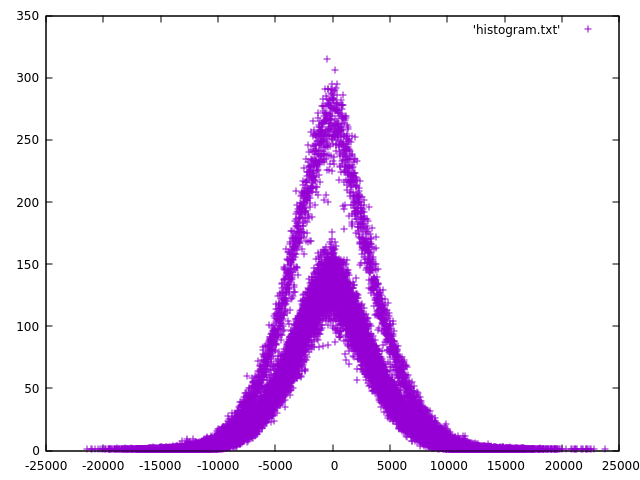
\includegraphics[width=\linewidth]{sample01_stereo_0.png}
  \end{minipage}%
  \begin{minipage}{.5\textwidth}
    \centering
    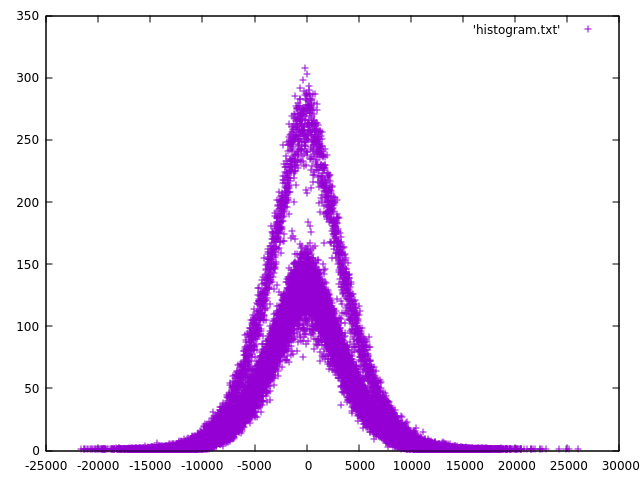
\includegraphics[width=\linewidth]{sample01_stereo_1.png}
  \end{minipage}
  \caption{Histogram of sample01.wav in the original format - channels 0 and 1.}
  \label{fig:histogram_stereo}
  
  \centering
  \begin{minipage}{.5\textwidth}
    \centering
    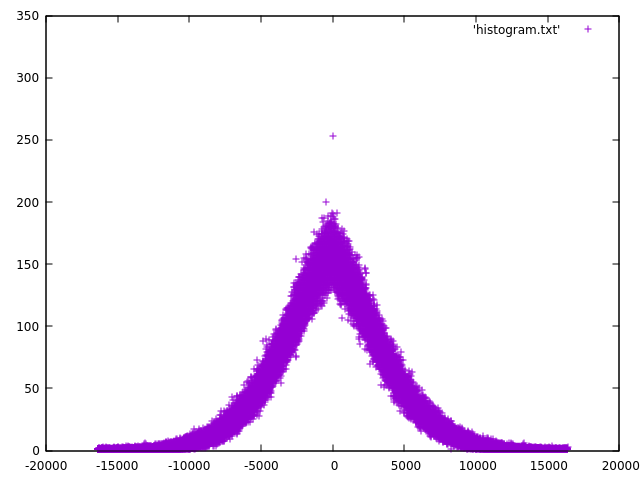
\includegraphics[width=\linewidth]{sample01_16_1.png}
  \end{minipage}%
  \caption{Histogram of sample01.wav after its conversion to mono (1 channel only).}
  \label{fig:histogram_mono}
\end{figure}

It is clear that the mono conversion affected the way the music file is 
represented, although it maintains a high fidelity to the original music. 
When analyzing Figures \ref{fig:histogram_stereo} and \ref{fig:histogram_mono}, 
the first thing we notice is the disappearance of the gap present in both 
channels of the stereo signal. 
This gap exists because the music has that frequency registry - note that each 
value in the x axis has one and only one y value -, so for this gap to occur 
close frequencies must have very different counts. 
When converting to mono, it is natural that this gap disappear, since it is 
necessary to take both sample channels and obtain their average.
If for one channel the value is in the top curve and for the other it's on the 
bottom curve, their average will be placed in the middle.
If this happens enough times, the gap is closed with the average values. 

\newpage
Another interesting phenomenon observed from these figures is that, in the mono 
signal, the number of occurrences decreases a bit. 
This once again can be explained by interpreting the mono conversion process: 
as each pair of samples will be aggregated into one, all the frequencies that 
occur very frequently have a high probability of being paired with each other, 
spreading the frequency counts in the way we see in Figure \ref{fig:histogram_mono}.

\begin{figure}[H]
  \begin{minipage}{.5\textwidth}
    \centering
    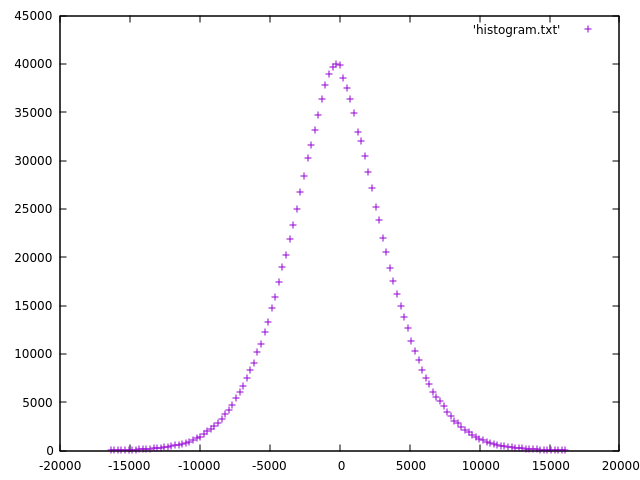
\includegraphics[width=\linewidth]{sample01_8_1.png}
    \caption{{8 bits, no reduction}}
    \label{fig:8_no}
  \end{minipage}
  \begin{minipage}{.5\textwidth}
    \centering
    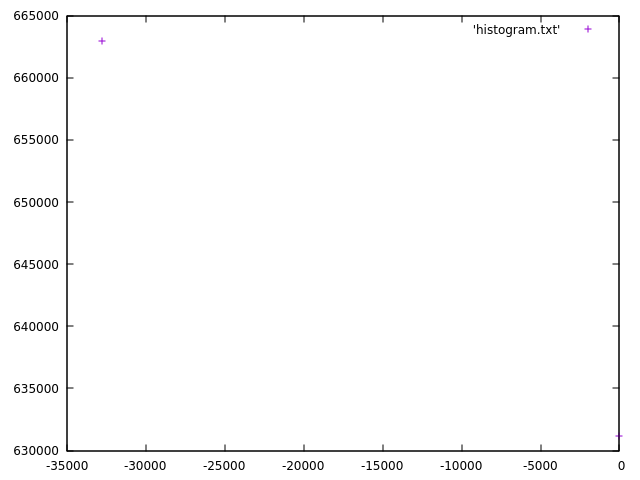
\includegraphics[width=\linewidth]{sample01_1_1.png}
    \caption{{1 bit, no reduction}}
    \label{fig:1_no}
  \end{minipage}
  \begin{minipage}{.5\textwidth}
    \centering
    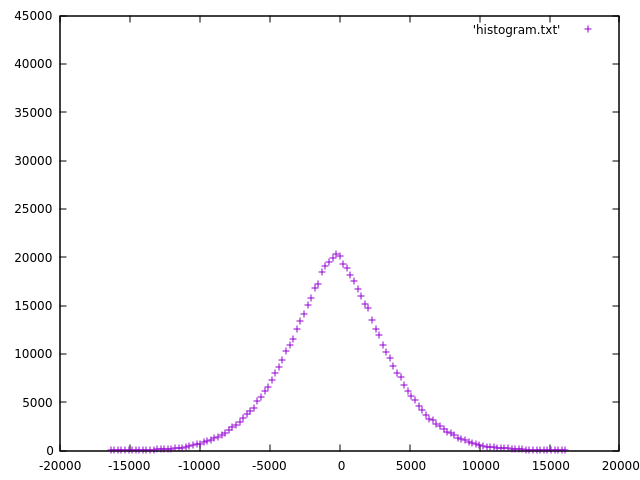
\includegraphics[width=\linewidth]{sample01_8_2.png}
    \caption{{8 bits, 2 reduction}}
    \label{fig:8_2}
  \end{minipage}
  \begin{minipage}{.5\textwidth}
    \centering
    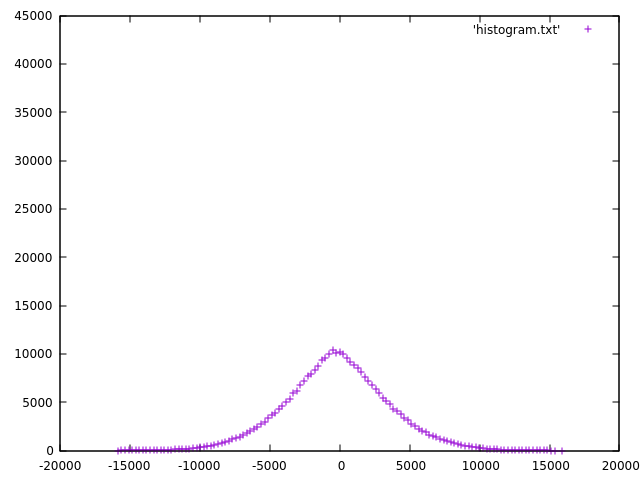
\includegraphics[width=\linewidth]{sample01_8_4.png}
    \caption{{8 bits, 4 reduction}}
    \label{fig:8_4}
  \end{minipage}
\end{figure}

Figures \ref{fig:8_no}, \ref{fig:1_no}, \ref{fig:8_2} and \ref{fig:8_4} depict 
two different studies: 
the first two dedicated to varying the quantization bit size;
the last two dedicated to varying the sampling rate reduction amount. 

The first two figures represent the histograms of the music segment 
\texttt{sample01.wav} quantized with 8 and 1 bits, respectively, and without a 
reduction of the sampling rate. 
A clear takeaway from these figures is that Figure \ref{fig:8_no} has a lot 
more frequencies than the other, which contains only two values.
Also, the frequency count values in Figure \ref{fig:1_no} are considerably higher. 
This behavior was to be expected, since when quantizing a signal we intend to 
decrease the number of bits required to represent each value, discarding the less 
significant values; for that reason, when using 1 bit to quantize the signal, 
there should be 2 resulting values, one in case the most significant bit is 1 and 
another if the bit is 0, and between them there should be all the samples 
present in the original signal. 

Theoretically speaking, it is possible to encounter $2^{b}$ values/levels, being 
{\it b\/} the number of bits used to quantize the signal.
However, in reality this number is not always observed since the original signal 
can have values that generate every level. 

In relation to the Figures \ref{fig:8_2} and \ref{fig:8_4}, which represent the 
reduction sampling rate factor behavior over a mono signal, quantized with 8 bits 
of the \texttt{sample01.wav} music, it is observable that the higher the reduction
the lower the count values become. 
This is directly related to the sampling reduction algorithm implementation, 
which aggregates as many samples the user indicated, i.e. if the user gave 4 as 
the reduction factor the algorithm will then aggregate every 4 samples, creating 
a 4:1 ratio and decreasing the sampling rate to 25\% of the original. 
This in turn will imply that the number of frequency count values will decrease,
since there are less values but also due to the aggregation: if there are very 
common frequencies, those occurrences end up distributed between other frequencies. \\

The C++ scripts mentioned in this chapter all use \texttt{libsndfile}, a C 
library used for reading and writing files containing sampled sound \cite{libsndfile}.
This was proposed on the assignment and allowed us to read and manipulate the 
audio files for more complex tasks.

\newpage
\section*{2. Data Processing}

Once we were capable of visualizing the data, we proceeded to actually doing 
something useful with it.
In this chapter we explain the implementation of the program \texttt{wavquant.cpp},
responsible for reducing the number of bits used to represent each audio sample.
The implementation of the formulas presented on the assignment's description for
the signal-to-noise ratio and the energies of the signals and noises is described
as well, along with the computation of vector quantization codebooks of audio files.

\subsection*{2.1. Uniform Scalar Quantization}

The idea behind a uniform scalar quantization (USQ) is the reduction of bits 
used to represent a signal.
Its usage has an instrinsic tradeoff between signal quality and memory space
required to store the information.
We do not get into much detail regarding the mathematics behind this process, 
but we make available a figure taken from a presentation from the Stanford 
University \cite{stanford} that helps visualizing the outcome of applying the 
USQ to a signal.
Figure \ref{fig:quantization} contains a signal presented in blue and the outcome
of the signal after it is quantized is presented in red. 
The figure also contains the quantization error variation on
the second plot.

\begin{figure}[H]
  \centering
  \begin{minipage}{\textwidth}
    \centering
    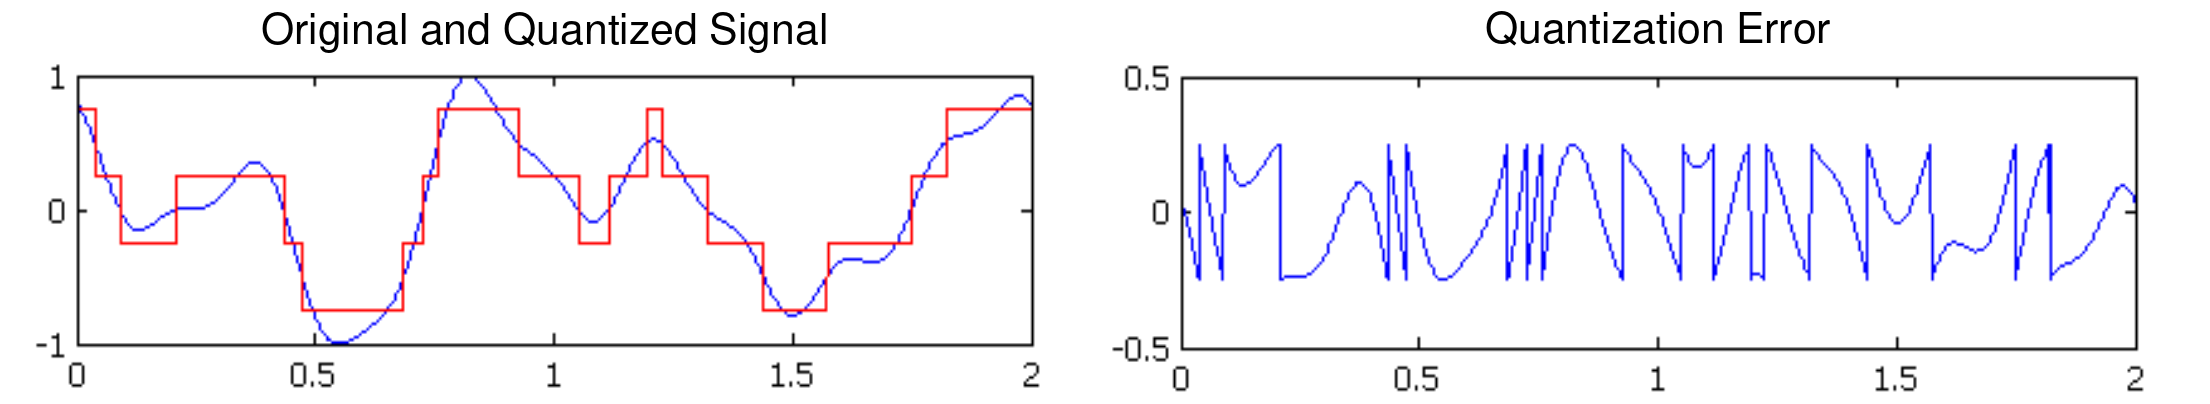
\includegraphics[width=\linewidth]{stanford_quantization_wide.png}
  \end{minipage}%
  \caption{Example of a quantized waveform.}
  \label{fig:quantization}
\end{figure}

It is \texttt{wavquant.cpp} that is responsible for this process.
As we have seen in Section 1.2, the script accepts two optional parameters:
\texttt{quantSize} defines the number of bits to be used to represent the audio 
fragment given as input (ideally, this value should be less than of the original 
source); \texttt{reductFactor} defines the number of times the user would like 
to reduce the total number of values of the audio signal.
This reduction factor works by calculating the average between \texttt{n} values, 
where \texttt{n = reductFactor}, and doing this for all values from the segment.
The result is a signal with \texttt{n} times less values (samples).

\newpage
\subsection*{2.2. Error Calculation}

A signal-to-noise (SNR) ratio compares a level of signal power to a level of 
noise power. 
Higher numbers generally mean a better specification, since there is more useful 
information (the signal) than there is unwanted data (the noise).

In \texttt{wavcb.cpp} we calculate this ratio, along with the maximum absolute 
error per sample. The SNR is defined as stated in equation \ref{eq:1}, taken 
from the assignment's description.

\begin{equation} \label{eq:1}
  SNR = 10 log_{10} \frac{E_{s}}{E_{n}} (dB)
\end{equation}

Here, $E_s$ is the energy of the signal, given by $E_s = \sum_{k} x_k^2$, and
$E_n$ is the energy of the noise, given by $E_n = \sum_{k} (x_k-\bar{x}_k)^2$,
where $x$ is the values from the audio segment.
The maximum error is defined in equation \ref{eq:2}, derived from the noise 
energy equation.

\begin{equation} \label{eq:2}
  error = |x_k-\bar{x}_k| \Leftrightarrow 
  max(error) = max(|x_k-\bar{x}_k|)
\end{equation}

In practice, the error of a quantization tells us how distant from the original
signal is the quantized one.
Figure \ref{fig:quantization} shows an example of how this error looks like.

However, for the following assignment tasks, we determined that the energy of
the noise would be more useful to us.
One way to compare audio fragments would be through the signal-to-noise ratios;
But we found that the only calculations actually required are of the noise 
energies as they work as the distances between two samples.
By focusing on these values, not only do we save processing time, but we are
also able to compare input audio segments to quantization codebooks already 
present in a program to determine the similarity between samples (and 
consequently between segments). These codebooks are explained in this next section.

\subsection*{2.3. Vector Quantization Codebook}
\label{sec:vctQuantCB}

Each music from the datasets is represented as a sequence of samples, where each 
sample is a singular frequency (if the file is in mono) or the pair of frequencies 
(one per channel, if the file is in stereo) that was registered in that exact second.
What a codebook is is basically an abstract representation of the overall 
sequence of samples.

In the context of our project, we integrated the concept of clusters to represent 
a given number of samples.
The base idea of this clustering is that similar data entities should have similar 
properties and can therefore be aggregated in a group.
On the other hand, data entries that differ significantly from each other
have properties considerably different as well, implying that they should belong 
to different groups \cite{clustering}. 

\newpage
Dividing the totality of samples present in each music into vectors with 'x' 
samples and representing them as points in a multidimensional vectorial space -  
as seen in Figure \ref{fig:pointsEx} - enables us to better comprehend the 
structure of the clusters.  
Geometrically speaking, clusters can be directly identified by the close 
grouping of the multidimensional points, since each axis represents a data 
property and similar points with similar properties stay closer to each other. 

By taking advantage of this natural grouping, clustering algorithms try to find 
points that represent the several data groups in a useful way, usually 
corresponding to the middle point of each group, known as centroid.

\begin{figure}[H]
  \centering
  \begin{minipage}{\textwidth}
    \centering
    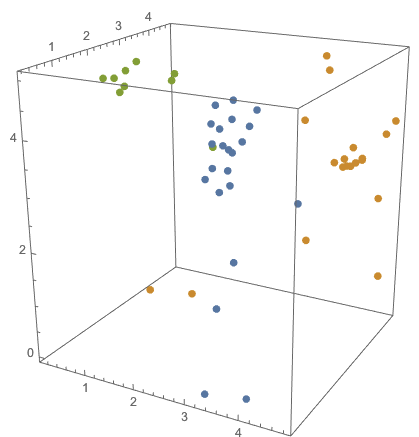
\includegraphics[width=0.4\linewidth]{pointsEx.png}
  \end{minipage}%
  \caption{Example of a 3-D visualization of point clusters.}
  \label{fig:pointsEx}
\end{figure}

So, in short, our interest in using such algorithms lies in the applicability of 
converting audio files into multidimensional clusters so that the most likely
cluster a new audio segment belongs to can be more easily identified.
A codebook is defined by the clusters that resulted from the process of mapping
the input audio file to its multidimensions.

In our implementation we used the K-Means Clustering algorithm, one of the 
most well-known clustering algorithm \cite{clustering}. 
K-Means was considered a good approach because it is relatively simple to 
implement and fast to execute, as it only requires the calculation of the 
distance between a given point and all existing centroids. 

The way it works is as follows.
The code starts by doing the already mentioned music partition in different 
blocks/vectors of a given size provided by the user;
Then the algorithm chooses, in a random fashion, an number of centroids given 
{\it a priori\/};
Once the pre-processing is done, the main algorithm begins calculating the 
closest centroid for each vector, and then updates each centroid by calculating 
the middle point of the points assigned to that specific centroid - this is 
repeated as many times as necessary for the error delta, i.e. the error between 
each iteration, to be lower than a given threshold specified by the user. 

The script \texttt{wavcb.cpp} is the implementation of this algorithm.
It enables the creation of a codebook for a given music by following the format 
below:

\begingroup
\addtolength\leftmargini{-0.4in}
\begin{quote}
\begin{verbatim}
$ ./wavcb inputFile blockSize overlapFactor errorThreshold
  numRuns outputFile
\end{verbatim}
\end{quote}
\endgroup

{\it InputFile\/} is the path to the .wav music whose codebook is to be constructed.
{\it BlockSize\/} is the value used as the size (number of samples) of the blocks 
in which the audio file is split.
{\it OverlapFactor\/} corresponds to the factor (a value between 0 and 1) that 
each block will be overlapped with the previous block; the bigger the overlapping
percentage is, the better the music is represented in the multidimensional space.
{\it CodebookDir\/} is the path to the directory containing the 
preprocessed codebooks of the music dataset.
{\it ErrorThreshold\/} is the maximum error that is allowed to exist in the last 
iteration; below this threshold, the centroids are no longer being adjusted in a 
worthwhile manner.
{\it NumRuns\/} is the number of times the K-Means algorithm will run to find 
the best local minimum; each run is initialized with the centroids in different 
positions.
At last, {\it outputFile\/} is the path to the file were the codebook will be stored. \\

Although quite flexible, K-Means has some disadvantages.
The most significant to our needs are the fact that it is necessary to insert the 
number of centroids to take in consideration which, in many situations, is not 
the best option, since the main purpose of using clustering is to get some 
insights about the data, preferring that the algorithm finds the number of 
centroids by itself; also, as K-Means' centroids start from a random starting 
position that is different each time it is executed, this makes it non-deterministic
and therefore not optimal as it can converge into a local minimum.
This last issue is dealt with in our solution by running K-Means several times to 
gain access to several local minimums and then choose the best one. 
As it is stated above, the number of times it is executed is defined by {\it numRuns\/}.

\newpage
\subsection*{2.4. Codebook Parallel Processing}

As audio files get longer, the number of frames per file increases and 
consequently so does the number of blocks that will be extracted from them.
Furthermore there is the overlapping factor detail, which increases even more 
the total number of blocks.
This high number of blocks brings computational time implications since, on the 
blocks classification step of the K-Means algorithm, each centroid has to be 
compared with each block and the closest centroid for each block must be determined.

Even though K-Means is considered a fast clustering algorithm, if given a 
considerable number of data entries, it is understandable that it starts to 
become cumbersome. 
To deal with this effect, we introduced parallelism into the process.
Practically speaking this means that we divide the blocks into groups and create
threads responsible for them and the calculation of the closest centroid.
To prevent having to create complex synchronization mechanisms, each thread 
stores the association between blocks and the closest centroids on different 
data structures and then the main thread is in charge of reading from those to 
recalculate the centroids.

As mentioned in the previous section, we deal with one of the K-Means algorithm's
disadvantages by testing it several times with different centroid initializations.
It is needless to say that this also slows down the algorithm.
To ease this, each K-Means run can be assigned to a thread, allowing to execute 
several runs at the same time.
In terms of implementation it implies some synchronization mechanisms, so the 
main thread knows when a run was completed and to manipulate the structure to 
store the centroids plus the associated error calculated on each run.

Figure \ref{fig:threading} is a visual representation of the execution flow of 
generating a codebook. 
The two independent time axis correspond to executing without additional threads 
and with 2 threads in each parallelization point.
Note that this is not an exact time representation and is ment only to illustrate
the advantage of multithreading. 

\begin{figure}[H]
  \centering
  \begin{minipage}{\textwidth}
    \centering
    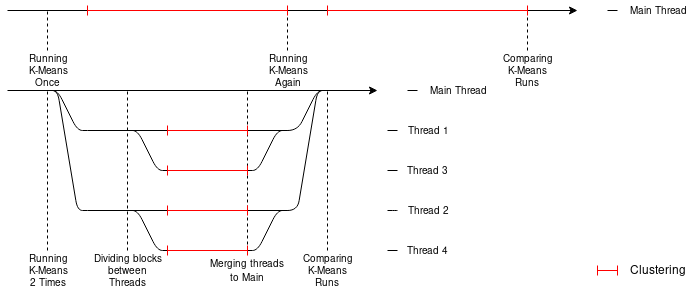
\includegraphics[width=0.95\linewidth]{threading.png}
  \end{minipage}%
  \caption{Visual representation of the execution flows with and without threading.}
  \label{fig:threading}
\end{figure}

\newpage
\section*{3. Automatic Music Identification}

The program \texttt{wavfind.cpp} is the application of the previous scripts on a 
program with a specific purpose.
WAVFind is meant to interpret a mono audio sample and attempt to identify which music 
from a database it belongs to.
In this chapter we discuss our solution, the consequences of varying the 
parameters passed to it and the quality of the results.

\subsection*{3.1. Most Probable Music}

The idea of WAVFind is very similar to the well known mobile app Shazam 
\cite{shazam} - a user plays a sound, the app listens to it, processes it and
determines the most probable music that sound belongs to.
Shazam has a large infrastructure, counting on online real-time music detection,
a nice user interface with access to the smartphone's microphone, and a variety
of other features.
We, on the other hand, focus on the functional end of this idea, implementing
it as a command line program with a limited dataset of known musics and with
the capacity to receive audio segments as input through their respective paths 
on the computer running the command.

To execute this command, one needs to use the following format:

\begingroup
\addtolength\leftmargini{-0.4in}
\begin{quote}
\begin{verbatim}
$ ./wavfind inputFile blockSize overlapFactor codebookDir
\end{verbatim}
\end{quote}
\endgroup

All arguments are mandatory and most of them we have seen on previous commands. 
{\it InputFile\/} is the path to the .wav audio whose origin music is to be identified.
{\it BlockSize\/} is the value used as the size of the blocks in which the audio 
segment is split; this value must be the same size used when the codebooks of 
the music dataset were built.
{\it OverlapFactor\/} corresponds to the factor (a value between 0 and 1) that 
each block will be overlapped with the previous block.
At last, {\it codebookDir\/} is the path to the directory containing the 
preprocessed codebooks of the music dataset.

The dataflow of the program is as follows:
first, the {\it inputFile\/} is validated and its information is extracted; 
then, it is split into blocks with size according to the parameter {\it blockSize\/}; 
now, for each codebook present in the {\it codebookDir\/}, each segment block 
is compared to each codebook block by calculating the $E_n$ (noise energy) 
between the two;
here, the minimum $E_n$ of each segment block is summed to a cumulative total
that represents the error between the segment and the codebook;
as this cumulative error is calculated for all codebooks, we then check which 
codebook returned the smallest error and assign it as the most similar to the
given audio segment.
This smallest error is determined iteratively - as each codebook is processed, 
we compare its cumulative error to the previous one and keep the smallest.
The identified codebook's is finally printed onto the console (as its name is 
supposed to identify the music it belongs to).

Now, for the program to work properly, there are a few prerequisites.
First of all, the program must have access to the codebook dataset.
The process of creating codebooks is neither trivial nor short-lasting, so to 
have access to the audio dataset is not enough.
Next, the audio segments passed as input files must contain only one signal 
channel (mono).
This restriction reduces the complexity of the comparison process, with the
obvious tradeoff of reducing the quality of the audio.
On the other hand, in a real case scenario (like with Shazam), the user would
usually record audio fragments from external sources such as speakers; so, to 
consider characteristics related to stereo files in the music identification 
process could lead to deceiving the program as the recording could fail in 
distributing the collected information to the proper channels.

\subsection*{3.2. Parameters Variation}

In this section we present some results of executing WAVFind for a few samples
from the datasets, explaining the experiences done with variations to the 
parameters passed to the command and their consequences.

The first experiment conducted regarded the effects of the overlapping factor 
and of the blocks' size on the accuracy of the results.
For this particular study, the use of the larger dataset did not bring any 
advantages so we used only the samples from the initial dataset.
The applied method focused on fixing all the parameters at meaningful values and
varying either the overlapping factor or the block size so that conclusions 
could be retrieved from the results of testing the identification capabilities 
of WAVFind.

The way we tested the samples was through a shell script \texttt{evaluateCodebooks.sh}
that randomly chooses one of the samples and also randomly chooses a small portion
of that file and then executes \texttt{wavfind.cpp} for that portion and returns
the correct answer along side with WAVFind's guess (it repeats this process as 
many times the user wishes). 
It is up for the user to manually check whether the guesses were correct or not.

The audio files were first preprocessed and converted to mono files with a 
quantization of 8 bits and no reduction factor.
The first codebooks were built with blocks of size 800, an error threshold of 
0.01 and with K-Means being run twice.
Five codebook folders were created, each containing the codebooks of all audio
segments of the initial dataset, but created with different overlapping factors:
0.00, 0.10, 0.25, 0.50 and 0.75. 
\texttt{EvaluateCodebooks.sh} was executed 10 times for each codebook folder,
and each execution ran 10 tests.
The average values of the 10 executions were then calculated.
The results are presented in Table \ref{tab:overlapFactor}.

\begin{table}[H]
  \begin{center}
    \begin{tabular}{c|c}
      \textbf{Overlapping Factor} & \textbf{Score}\\
      \hline
      0.00 & 6/10\\
      0.10 & 8/10\\
      0.25 & 9/10\\
      0.50 & 9/10\\
      0.75 & 10/10\\
    \end{tabular}
  \end{center}
  \caption{Test results on varying the overlapping factor between blocks.}
  \label{tab:overlapFactor}
\end{table}

The second group of codebooks were built with an overlapping factor of 0.1, an 
error threshold of 0.01 and with K-Means being run twice.
Five codebook folders were created, each containing the codebooks of all audio
segments of the initial dataset, but created with different block sizes:
50, 100, 400, 800, 1600. 
\texttt{EvaluateCodebooks.sh} was once again executed 10 times for each codebook
folder, and each execution ran 10 tests.
The average values of the 10 executions were then calculated.
The results are presented in Table \ref{tab:blockSize}.

\begin{table}[H]
  \begin{center}
    \begin{tabular}{c|c}
      \textbf{Block Size} & \textbf{Score}\\
      \hline
      50 & 3/10\\
      100 & 5/10\\
      400 & 6/10\\
      800 & 9/10\\
      1600 & 9/10\\
    \end{tabular}
  \end{center}
  \caption{Test results on varying the blocks' sizes.}
  \label{tab:blockSize}
\end{table}

Our second study was dedicated to finding the best number of centroids in relation
to the total number of blocks for the best performance of WAVFind.
Since the definition of the number of centroids is directly related to the number
of blocks and is not a parameter chosen by the user executing our commands,
we had to find another way of testing the variation of this aspect.

To do this, we introduced an auxiliar parameter, which we called alpha, that is 
present in the assignment of a value to the number of centroids 
$numCentroids = alpha . len(blocks)$, where {\it len(blocks)\/} is the total 
number of blocks.
This implies that the longer the audio files are, the more centroids are needed
on the K-Means algorithm for the music identification process.

The audio files were first preprocessed just like in the previous study.
The generated codebooks were built with blocks of size 800, an overlapping 
factor of 0.3, an error threshold of 0.01 and with K-Means being run twice.
Four codebook folders were created, each containing the codebooks of all audio
segments of the initial dataset, but created with different alpha values:
0.2, 0.4, 0.6, 0.8.
\texttt{EvaluateCodebooks.sh} was used one more time, this time executed only 
once but running 100 tests (in practice, this worked the same way, as in the end 
we rounded the results to the same scale).
The results are presented in Table \ref{tab:numcentroids}.

\begin{table}[H]
  \begin{center}
    \begin{tabular}{c|c}
      \textbf{Alpha} & \textbf{Score}\\
      \hline
      0.2 & 7/10\\
      0.4 & 6/10\\
      0.6 & 5/10\\
      0.8 & 5/10\\
    \end{tabular}
  \end{center}
  \caption{Test results on varying the number of centroids (through alpha).}
  \label{tab:numcentroids}
\end{table}

The last study was related to multithreading and the benefits of parallelism.
The goal was to build codebooks for musics using different strategies and
determining what is the fastest alternative.
It is important to state that, due to the shortage of time for conducting this 
test for all available musics, we focused on one music from the larger dataset.
The chosen music was {\it Don't Worry Be Happy\/}, by Bob Marley, with a disk 
space usage of 51.1MB, converted to mono, quantized with 8 bits with a reduction 
factor of 5.
The remaining parameters were once again kept at fixed values, with the blocks'
size equal to 800, the overlapping factor at 0.1, an error threshold of 0.01 and
the K-Means algorithm executed twice.
The computer used to perform this study was an SSD, i7 with 4 cores and 16GB of RAM.
The times taken for building the codebooks are presented in Table \ref{tab:multithreading}.
Note: most of the elements of the first column contain two values, these 
correspond to the number of threads used for all K-Means runs and to the number
of threads distributed with blocks for clustering.

\begin{table}[H]
  \begin{center}
    \begin{tabular}{c|c}
      \textbf{Number of Additional Threads} & \textbf{Execution Time}\\
      \hline
      Main Thread Only & 40 min. 06 sec.\\
      1, 2 & 33 min. 03 sec.\\
      1, 4 & 29 min. 54 sec.\\
      2, 1 & 31 min. 25 sec.\\
      2, 2 & 27 min. 36 sec.\\
      2, 3 & 21 min. 22 sec.\\
    \end{tabular}
  \end{center}
  \caption{Test results on varying the number of threads during codebook construction.}
  \label{tab:multithreading}
\end{table}

\subsection*{3.3. Results Discussion}

In this section we analyse the results of the previous studies done on the 
developed programs and reach some conclusions regarding the optimal parameters.

From the results of the first study, we concluded that introducing an overlapping 
between blocks does benefit the program's accuracy.
However, a high value does not always mean a better result.
Considering the increase in execution time with higher overlapping factors, we 
saw that 0.25 was a good balance between effectiveness and speed.
Although 0.75 had a 10/10 score, it took too long to return the results so we 
considered it not advisable for usability reasons.\\

As for the block size, we understood that blocks too small makes it harder to 
define well delimited clusters (as there are less dimensions to characterize the
points), reducing the accuracy of the algorithm.
Basically we have another case of a tradeoff between execution speed and accuracy.
With this in mind, we found what we believe to be an approximation to a balance
between these two perspectives, which was a value around 800. 
Above this value, the gains in performance were not relevant enough for the 
increase in execution time. \\

Our second study was the toughest of them all.
What we intended from it was to achieve a good estimation of the ideal percentage
of centroids in relation to the number of blocks of the audio files.
However, we found a contradiction on the results we were not entirely able to 
comprehend.
One possible explanation for the reduction in accuracy with higher alpha values
is the existence of the overfitting phenomenon. 
However, in this particular case, overfitting should not be an issue.
Although not presented on the results table, we saw that codebooks with more
centroids classify better the musics (in terms of errors), as the errors decrease
as the number of centroids is increased.
But this is not what we see in the results.
Due to the lack of time to increase the depth of this study, we could only 
conclude that the results suggest that the number of centroids must be a lot 
smaller than the number of blocks. 
For future work, we found the need to test the program and the datasets for 
different alpha values and carefully analyse the results again in order to 
reach more solid conclusions regarding the variation of the number of centroids. \\

The results on multithreading were a bit difficult to interpret, as we must take 
in consideration that the performance also depends on the number of available 
processing cores in the hardware executing our code, i.e. computers with less
available cores than the number of threads given will not benefit from them as much.
However, it is possible to see that, on average, multithreading will be faster
than using one thread only.
This is not linear, i.e. more threads does not necessarily mean more speed, but
there is a clear decrease in execution time from the first alternative to the 
remaining.

In addition, the results seem to suggest that the external threads (where we 
assign one thread per K-Means run) seem to be more effective than the internal
threads (where we distribute the blocks amongst threads for clustering).
It is supposed to be like so, as the internal threads only improve block 
classification, but the centroids remain updated sequentially.

Another conclusion we believe to be true and is verified by the results is that
the best alternative is to combine both forms of multithreading in order to get
the advantages of both.

\newpage
We'd like to mention that all of the studies were conducted simultaneously,
distributing the tasks amongst our group.
This means that, for each study, the values for the parameters kept static were
chosen according to personal estimations, with the group consensus and within
reasonable boundaries.
Also, since they were not made sequentially, the combination of the best values
of all studies does not necessarily mean that we achieve the best combination for
the most accurate program; rather, the studies only deliver us good guidelines
in case we desired to actually deploy the program.

\section*{Conclusions}

After completing the assignment, we drew a few conclusions regarding our 
solutions and the applicability of algorithms such as the K-Means to solving
problems like music identification.

First of all, the existance of initial code with a few features already 
implemented was very helpful during the initial stages of development, as they 
served as the basis of our manipulations of the audio files.

Also, it was very rewarding to develop our own K-Means implementation, without 
the use of external Python libraries. 
Not only did this made its manipulation and control easier, but it also made us 
understand far better the way it actually works.

The introduction of multithreading in our solutions was very interesting as well,
as it was the first time we were able to compare two forms of distributing work
amongst threads and see their individual and joint effects on the solution's 
performance.

Regarding our satisfaction with the delivered code, we considered fairly well 
structured, although this time the code was not based on object-oriented classes
as it was purely scripting programming.
For the final versions, each script does what it is supposed to with great 
flexibility and ease of use.
The overall performance of the final program WAVFind is very positive for both
datasets, rounding the 90\% of accuracy with the parameters chosen with 
consideration to the results collected from our studies.

In terms of code organization and readability, we made sure our 
repository was as well structured as possible and our code properly commented
and documented.
The base folder contains a {\it README\/} file for basic instructions and a 
{\it Makefile\/} to make the compilation process easier.
All code is in the {\it src\/} folder.

\newpage
\begin{thebibliography}{9}
  \bibliographystyle{Science}

  \bibitem{trab1}
    Armando J. Pinho,
    \textit{AIT: Lab Work no.2},
    University of Aveiro,
    2019/20.
  
  \bibitem{gnuplot}
    H.B. Broeker, G. Clark, L. Hecking and E. Merritt,
    \textit{Gnuplot: graphing utility},
    \url{http://www.gnuplot.info/} ,
    May 2019,
    [accessed in: November 2019].

  \bibitem{libsndfile}
    Free Software Foundation,
    \textit{GLibsndfile API},
    \url{http://www.mega-nerd.com/libsndfile/api.html} ,
    April 2013,
    [accessed in: November 2019].

  \bibitem{stanford}
    Bernd Girod,
    \textit{Image and Video Compression: Quantization},
    \url{https://web.stanford.edu/class/ee398a/handouts/lectures/05-Quantization.pdf} ,
    [accessed in: November 2019].

  \bibitem{shazam}
    Apple Inc.,
    \textit{Shazam for iOS \& Android},
    \url{https://www.shazam.com/apps} ,
    [accessed in: November 2019].

  \bibitem{clustering}
    George Seif,
    \textit{The 5 Clustering Algorithms Data Scientists Need to Know},
    \url{https://towardsdatascience.com/the-5-clustering-algorithms-data-scientists-need-to-know-a36d136ef68} ,
    [accessed in: November 2019].

\end{thebibliography}

\clearpage

\end{document}




















